\documentclass{beamer}
\setbeameroption{show notes}


\mode<presentation>
{
\usetheme{Pittsburgh}      % Madrid, Montpellier, Pittsburgh, Rochester, boxes
\usecolortheme{dove} 	% beaver, crane, dolphin, dove, lily, orchid, seagull, seahorse
\usefonttheme{default}  % or try serif, structurebold, ...
\setbeamertemplate{navigation symbols}{}
\setbeamertemplate{caption}[numbered]
}

\usepackage[portuguese]{babel}
\usepackage[utf8x]{inputenc}
\usepackage{multirow}
\usepackage{ragged2e}
\usepackage{textpos}
\usepackage[export]{adjustbox}
\usepackage{caption}
\justifying
\usepackage{pifont}
\newcommand{\xmark}{\ding{55}}%
\usepackage{tikz}
\usepackage[skins]{tcolorbox}
\usetikzlibrary{arrows,positioning} 
\usetikzlibrary{matrix}
\usetikzlibrary{fadings,shapes,arrows,chains,backgrounds,calc,arrows,arrows.meta,shadows,shapes.geometric, fit, positioning, circuits.logic.US, circuits, decorations.markings, arrows.meta}

\setlength{\parindent}{0.5cm}
%%%%%%%%%%%%%%%%%%%%%
% Títulos e etc
\title[Apresentação Final]{Co-processador da Transformada para o Codificador de Vídeo AV1}
\subtitle{Apresentação Final}
\author[M. Inocêncio]{Miguel Inocêncio}
\institute[UA]{Universidade de Aveiro\\ 
				Instituto de Telecomunicações}
\date{18/12/2019}
%\titlegraphic{
\includegraphics[height=1.5cm]{../ua.jpg}\includegraphics[height=1.5cm]{../IT.png}}

\begin{document}

%%%%%%%%%%%%%%%%%%%%%
% Página Inicial
\begin{frame}
	\titlepage
\end{frame}

%%%%%%%%%%%%%%%%%%%%%
% Table of Contents
\begin{frame}{Conteúdos}
	\tableofcontents
\end{frame}

%%%%%%%%%%%%%%%%%%%%%%
% Introdução
\section{Introdução}

\begin{frame}
	\frametitle{Consumo de Vídeo}
       \begin{columns}
              \column{\textwidth}
                     \begin{figure}[h]
                            \centering
                            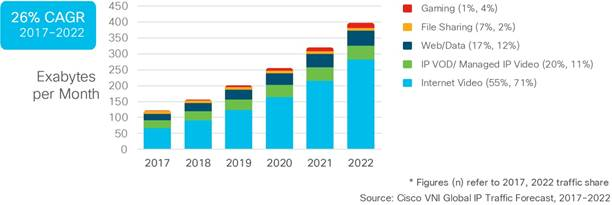
\includegraphics[width=\textwidth]{Figures/cisco.jpg}
                            \caption{Previsões da \emph{Cisco} para evolução de tráfico IP}
                            \label{fig:cisco}
                     \end{figure}
       \end{columns}
\end{frame}

\note[itemize]{
       \item Consumo de vídeo tem vindo a aumentar exponencialmente
       \item A Cisco prevê que para 2022 82\% do tráfico IP esteja dedicado à vizualização de vídeo
}

\begin{frame}
       \frametitle{Necessidade de Compressão de Vídeo}
       \begin{figure}[h]
              \centering
              \begin{tikzpicture}
    \makeatletter
    \tikzset{   len/.style={<->, line width=0.3mm, >=stealth'},
                to/.style={->, line width=0.8mm, >=stealth'},
                database/.style={
                    path picture={
                        \draw[very thick] (0, 1.5*\database@segmentheight) circle [x radius=\database@radius,y radius=\database@aspectratio*\database@radius];
                        \draw[very thick] (-\database@radius, 0.5*\database@segmentheight) arc [start angle=180,end angle=360,x radius=\database@radius, y radius=\database@aspectratio*\database@radius];
                        \draw[very thick] (-\database@radius,-0.5*\database@segmentheight) arc [start angle=180,end angle=360,x radius=\database@radius, y radius=\database@aspectratio*\database@radius];
                        \draw[very thick] (-\database@radius,1.5*\database@segmentheight) -- ++(0,-3*\database@segmentheight) arc [start angle=180,end angle=360,x radius=\database@radius, y radius=\database@aspectratio*\database@radius] -- ++(0,3*\database@segmentheight);
                    },
                    minimum width=2*\database@radius + \pgflinewidth,
                    minimum height=3*\database@segmentheight + 2*\database@aspectratio*\database@radius + \pgflinewidth,
                },
                database segment height/.store in=\database@segmentheight,
                database radius/.store in=\database@radius,
                database aspect ratio/.store in=\database@aspectratio,
                database segment height=0.1cm,
                database radius=0.25cm,
                database aspect ratio=0.35
            }

    \path[fill overzoom image={Figures/cat.jpg}] (0,0) node[minimum width=0.5\textwidth, minimum height=0.4\textheight, anchor=south west] (cat) {} rectangle (0.5\textwidth,0.4\textheight) {};
        \draw [len] ([xshift=-2mm] cat.south west) -- ([xshift=-2mm] cat.north west);
            \node at (cat.west) [rotate=90, yshift=5mm, font={\bfseries\large}] {720 px};
        \draw [len] ([yshift=2mm] cat.north west) -- ([yshift=2mm] cat.north east);
            \node at (cat.north) [yshift=5mm, font={\bfseries\large}] {1280 px};

    \node[database, label=below:24 GB, font={\bfseries\large}, database radius=1cm,database segment height=0.5cm, right=2cm of cat.east] (db) {};
        \draw[to] ([xshift=1mm]cat.east) -- ([xshift=-1mm]db.west) node [midway,above] {5 min.};
\end{tikzpicture}
       \end{figure}
\end{frame}

\note[itemize]{
       \item Enorme quantidade de dados gerados com a captura ou criação de vídeo
       \item Vídeo HD a 30 frames por segundo num espaço RGB de 8 bits por cor ocuparia 24GB em 5 minutos
       \item Para as resoluções que se desejam hoje em dia este problema seria ainda mais grave
       \item Necessidade de reduzir quantidade de informação precisa para reproduzir um vídeo
}

\begin{frame}[plain,t]
       \begin{center}
              \Huge \textbf{Codificação de Vídeo}\\ \vspace{1cm}
              \Large Remoção de informação de sequência de imagens, mantendo a capacidade de reprodução
       \end{center}
       \vspace{1cm}
       \begin{figure}[h]
              \centering
              \begin{tikzpicture} [y=1cm]
    \makeatletter
    \tikzset{   len/.style={<->, line width=0.3mm, >=stealth'},
                to/.style={->, line width=0.8mm, >=stealth'}
            }

    \foreach \x in {0,0.6,1.2,1.8}
        \draw[fill=green!80!black, draw=black] (0,\x) rectangle (3,\x+0.3);
    \foreach \x in {0.3,0.9,1.5,2.1}
        \draw[fill=red!80!black, draw=black] (0,\x) rectangle (3,\x+0.3);
    \node at (1.5,-0.2) [below, font={\bfseries\large}] {1940};

    \draw[to] (3.2,1.2) -- (4.5,1.2);
    \node[inner sep=0pt, anchor=west] at (4.7,1.2) (av1l) {
\includegraphics[width=3cm]{Figures/av1.png}};
    \node at (6.1,-0.2) [below, font={\bfseries\large}] {2018};
\end{tikzpicture}
       \end{figure}
\end{frame}

\note[itemize]{
       \item Levou ao conceito de codificação de vídeo
       \item Em prática desde os anos 40 com o interlaced scanning das televisões de raios catódicos
       \item Evolução do vídeo levou à evolução dos métodos de compressão (aumento da complexidade)
       \item Alliance for Open Media Video One ou AV1 apresenta grandes taxas de compressão, a custo de elevada complexidade
       \item Necessidade de software optimizado e arquiteturas de hardware eficientes
}

%%%%%%%%%%%%%%%%%%%%%%
% Sistemas de Codificação de Vídeo
\section{Sistemas de Codificação de Vídeo}

\begin{frame}
       \frametitle{Redundâncias}
       \begin{columns}
              \column{0.5\textwidth}
              \begin{figure}[h]
                     \centering
                     \begin{tikzpicture}[scale=0.7,>=triangle 60]
\tikzset{
    a/.style={->},
}    
    \draw [fill=lightgray] (0,0) rectangle (1,5);
    \draw [fill=lightgray] (1,4) rectangle (9,5);
    \draw[step=1cm,black,very thin] (0,0) grid (5,5);
    \draw[step=1cm,black,very thin] (5,4) grid (9,5);

    \node at (1.5,4.5) {A};
    \node at (2.5,4.5) {B};
    \node at (3.5,4.5) {C};
    \node at (4.5,4.5) {D};
    \node at (5.5,4.5) {E};
    \node at (6.5,4.5) {F};
    \node at (7.5,4.5) {G};
    \node at (8.5,4.5) {H};

    \node at (0.5,4.5) {I};
    \node at (0.5,3.5) {J};
    \node at (0.5,2.5) {K};
    \node at (0.5,1.5) {L};
    \node at (0.5,0.5) {M};

    \draw [a] (8,4) --(4,0);
    \draw [a] (7,4) --(3,0);
    \draw [a] (6,4) --(2,0);
    \draw [a] (5,4) --(1,0);
    \draw [a] (4,4) --(1,1);
    \draw [a] (3,4) --(1,2);
    \draw [a] (2,4) --(1,3);
\end{tikzpicture}
                     \caption*{Espaciais}
              \end{figure}
              \begin{figure}[h]
                     \centering
                     \begin{tikzpicture}[scale=0.75]    
    \coordinate (ycenter) at (2,3);
    \node[align=center] at (ycenter.north) {\textbf{Y}};
    \fill[gray!40] (0,0) rectangle (1,1);
    \fill[gray!70] (1,0) rectangle (2,1);
    \fill[gray!40] (2,0) rectangle (3,1);
    \fill[gray!70] (3,0) rectangle (4,1);
    \fill[gray!70] (0,1) rectangle (1,2);
    \fill[gray!40] (1,1) rectangle (2,2);
    \fill[gray!70] (2,1) rectangle (3,2);
    \fill[gray!40] (3,1) rectangle (4,2); 
    
    \coordinate (ccenter) at (7,3);
    \node[align=center] at (ccenter.north) {\textbf{Cb/Cr}};
    \fill[blue!80!black] (5,0) rectangle (6,1);
    \fill[blue!80!black] (6,0) rectangle (7,1);
    \fill[pink] (7,0) rectangle (8,1);
    \fill[pink] (8,0) rectangle (9,1);
    \fill[blue!80!black] (5,1) rectangle (6,2);
    \fill[blue!80!black] (6,1) rectangle (7,2);
    \fill[pink] (7,1) rectangle (8,2);
    \fill[pink] (8,1) rectangle (9,2);

\end{tikzpicture}
                     \caption*{Psico-Visuais}
              \end{figure}

              \column{0.5\textwidth}
              \begin{figure}[h]
                     \centering
                     \begin{tikzpicture}[scale=.7,every node/.style={minimum size=1cm},on grid,>=triangle 60]
		
    %slanting: production of a set of n 'laminae' to be piled up. N=number of grids.
    \begin{scope}[
            yshift=-83,every node/.append style={
            yslant=0.5,xslant=-1},yslant=0.5,xslant=-1
            ]
        % opacity to prevent graphical interference
        \fill[white,fill opacity=0.9] (0,0) rectangle (5,5);
        \draw[blue!40!black,very thick] (0,0) rectangle (5,5);%marking borders
        \filldraw[blue!30] (0.5,0.5) rectangle (1.5,1.5);
        \draw[gray, dashed] (0.5,1.5) -- (3.42,4.42);
        \draw[gray, dashed] (1.5,0.5) -- (4.42,3.42);
        \draw[gray, dashed] (0.5,0.5) -- (3.42,3.42);
        \draw[gray, dashed] (1.5,1.5) -- (4.42,4.42);
        %Idem as above, for the n-th grid:
    \end{scope}
    
    \begin{scope}[
    	    yshift=0,every node/.append style={
    	    yslant=0.5,xslant=-1},yslant=0.5,xslant=-1
            ]
        \fill[white,fill opacity=.9] (0,0) rectangle (5,5);
        \draw[black,very thick] (0,0) rectangle (5,5);

        \draw[blue!30] (0.5,0.5) rectangle (1.5,1.5);
        \filldraw[gray] (2.5,3) rectangle (3.5,4);

        \draw[->] (0.5,0.5) -- (2.5,3);
    \end{scope}

    \draw[-latex,thick](5.8,0)node[right]{Reference Frame}
    to[out=180,in=90] (3.4,-1);

    \draw[-latex,thick] (5.8,3) node[right]{Present Frame}
         to[out=180,in=90] (3.4,2);

    \draw[-latex,thick] (-5.5,2.2) node[left]{Motion Vector}
    to [out=0,in=180](-0.22,1.5);
\end{tikzpicture}
                     \caption*{Temporais}
              \end{figure}
              \begin{figure}[h]
                     \centering
                     \begin{tikzpicture}[iv/.style={draw,fill=red!50,circle,minimum size=20pt,inner
    sep=0pt,text=black},ev/.style={draw,fill=yellow,rectangle,minimum
    size=20pt,inner sep=0pt,text=black},scale=0.3, every node/.style={transform shape}]
    \node[iv]{31}
      child {node[iv]{18}
             child {node[iv]{11}  
                    child {node[iv]{6}
                           child {node[iv]{3}
                                  child {node[ev]{E(1)}}
                                  child {node[ev]{C(2)}}
                                 }
                           child {node[ev]{B(3)}}
                          }
                    child {node[ev]{D(5)}}
                    }
             child [missing]
             child {node[iv]{7}
             child {node[ev]{A(4)}}
             child {node[ev]{G(3)}}
                   }
            edge from parent node[above]{O}        
            }
      child [missing]
      child [missing]
      child {node[iv]{13}
             child {node[ev]{F(6)}}
             child {node[ev]{H(7)}}
            };
\end{tikzpicture}
                     \caption*{Código}
              \end{figure}
       \end{columns}
\end{frame}

\note[itemize]{
       \item Apesar da evolução, os princípios de base continuam os mesmos
       \item 4 tipos de redundâncias, a maioria causadas pela interpretação do olho humano
       \item Espaciais referentes à proximidade de pixeis proximos
       \item Temporais referentes à semelhança de pixeis em imagens consecutivas
       \item Psicovisuais referentes à perceção mais baixa da cor ou de detalhes
       \item Código, não sendo referente à imagem ou perceção, mas à representação dos símbolos em domínio digital
       \item Estas redundâncias são exploradas em vários estágios de um codificador de vídeo
}

\begin{frame}
       \frametitle{Modelo Básico de Codificador}
       \begin{figure}[h]
              \centering
              \begin{tikzpicture}[%
    >=triangle 60,              % Nice arrows; your taste may be different
    start chain=going right,    % General flow is top-to-bottom
    node distance=2.5cm,          % Global setup of box spacing
    every join/.style={norm},   % Default linetype for connecting boxes
    scale=0.7, every node/.style={transform shape}
    ]

\tikzset{
    base/.style={draw, on chain, on grid, align=center},
    proc/.style={base, rectangle, text width=1.6cm, fill=black!15, minimum height=1.5cm, minimum width=1.5cm,font={\bfseries}},    
    frame/.style={base, minimum height=1.5cm, minimum width=2cm, fill=blue!10, thick},
    sub/.style={base, circle, inner sep=0pt, radius=0.4cm, fill=black!10, minimum height=3.5ex, font={\bfseries}},
    spot/.style={circle, inner sep=0pt, radius=0.4cm, minimum height=2mm, draw},
    edge rectangle/.style={ to path={ rectangle (\tikztotarget)}},
    % coord node style is used for placing corners of connecting lines
    coord/.style={coordinate, on chain, on grid, node distance=6mm and 40mm},
    % Arrows 
    fforw/.style={->, thick},
    fback/.style={->, thick, red!75!black},
    aref/.style={<->, dashed, black!50},
    % -------------------------------------------------
    % Connector line styles for different parts of the diagram
    cascaded/.style = {%
    general shadow = {%
      shadow scale = 1,
      shadow xshift = -1ex,
      shadow yshift = 1ex,
      draw,
      thick,
      fill = blue!40},
    general shadow = {%
      shadow scale = 1,
      shadow xshift = -.5ex,
      shadow yshift = .5ex,
      draw,
      thick,
      fill =blue!40},
    fill = blue!40, 
    draw,
    thick,
    minimum width = 2cm,
    minimum height = 1.5cm},
    base
}    

%% Top row
\node [frame] (inframe) {Input\\Frame};
    \node [coord] (ni1) {};    
    \node [coord, right=2mm of inframe.east] (ni2) {};
\node [sub, right=2cm of ni1] (sub) {-};
    \draw [fforw] (inframe) -- (sub);
\node [proc] (T) {T};
    \draw [fforw] (sub) -- (T);
\node [proc] (Q) {Q};
    \draw [fforw] (T) -- (Q);
\coordinate (rq) at ($(Q.east)+(4mm,0)$);
\node [proc, right=1cm of Q.east] (EC) {Entropy\\Coding};
    \draw [fforw] (Q) -- (EC);
\coordinate (out) at ($(EC.east)+(4mm,0)$);
%\path (EC) to node [yshift=-1em] {Encoded\\Bitstream} (out);
    \draw [fforw] (EC) -- (out);

%% Reference
\node [cascaded, below=5cm of inframe] (ref) {Reference\\Frames};

%% Intra
\node [proc, below=1.5cm of ni1] (intra) {Intra\\Coding};
    \coordinate (ni3) at (ni2 |- intra);    
    \draw [fforw] (ni3) -- (intra);

%% Inter    
\node [proc,right=of ref] (inter) {Inter\\Coding};
    \node [coord, below=4.5cm of ni2] (ni4) {};
    \draw [fforw] (ni2) -- (ni4) |- ($(inter.west)+(0,5mm)$);
    \draw [fforw] ($(ref.east)+(0,-5mm)$) -- ($(inter.west)+(0,-5mm)$);

%% Selector
\coordinate (rintra) at ($(intra.east)+(5mm,0)$);
\node [spot, below=1cm of rintra, fill=black] (sintra) {};
    \draw [thick] (intra.east) -- (rintra) |- (sintra.north);

\coordinate (rinter) at ($(inter.east)+(5mm,0)$);
\node [spot, above=1cm of rinter, fill=black] (sinter) {};
    \draw [thick] (inter.east) -- (rinter) |- (sinter.south);

\path (sintra) -- (sinter) coordinate [midway] (intraintermid);
\node [spot, at=(sub |- intraintermid)] (sel) {};
\draw [dashed] ($(sel)+(-4mm,3.3mm)$) arc (140:220:5mm);
    \draw [fforw] (sintra) -- (sel);
    \draw [fforw] (sel) -- (sub);

%% Lower Row    
\node [sub, below=3.7cm of sel] (add) {+};
    \draw [fback] (sel) -- (add);
\node [proc] (T1) {$\mathbf{T^{-1}}$};
    \draw [fback] (T1) -- (add);
\node [proc] (Q1) {$\mathbf{Q^{-1}}$};
    \draw [fback] (Q1) -- (T1);
\coordinate (rq1) at ($(Q1.east)+(4mm,0)$);
    \draw [fback] (rq) -- (rq1) |- (Q1);
\node [frame, below=7.4cm of inframe] (recframe) {Reconstructed\\Frame};
    \draw [fback] (add) -- (recframe);
\end{tikzpicture}
       \end{figure}
\end{frame}

\note[itemize]{
       \item Processo começa com frame de entrada que é dividido em blocos
       \item Estágio de predição Intra ou Inter
       \item Bloco previsto subtraído por original
       \item Transformada é o foco do trabalho
       \item Avalia componentes de frequência
       \item Quantização avalia coeficientes de maior relevância para reconstrução de imagem
       \item codificador de entropia organiza símbolos segundo códigos de comprimento variável
       \item Loop de feedback para restaurar imagem do descodificador para uso nos estágios de predição
       \item Unidade de controlo escolhe quais as ferramentas de codificação a usar
       \item Descodificador faz operação inversa
}

\end{document}	